\subsection{Práctica 3}

\subsubsection{Puntos de operación amplificador multietapas desacoplado}

\begin{table}[h!]
\centering
\begin{tabular}{|c|c|c|c|c|c|c|c|c|c|}
\hline
\textbf{Transistor} & \textbf{\(Vc[V]\)} & \textbf{\(\varDelta Vc[V]\)} & \textbf{\(Vb[V]\)} & \textbf{\(\varDelta Vb[V]\)} & \textbf{\(Ve[V]\)} & \textbf{\(\varDelta Ve[V]\)} & \textbf{\(Re[\Omega]\)} & \textbf{\(\varDelta Re[\Omega]\)} \\ \hline
Q1 & 7.2 & 0.4 & -0.04 & 0.002 & -0.6 & 0.04 & 4700 & 470 \\ \hline
Q2 & 7.6 & 0.4 & -0.068 & 0.004 & -0.64 & 0.04 & 4700 & 470 \\ \hline
Q3 & 8 & 0.4 & 8 & 1 & 7.4 & 0.4 & 6800 & 680 \\ \hline
Q4 & 0.68 & 0.04 & -0.6 & 0.04 & -0.6 & 0.04 & 5000 & 500 \\ \hline
Q5 & 10 & 1 & 0.68 & 0.04 & 0.2 & 0.01 & 20 & 1 \\ \hline
Q6 & -10 & 1 & -0.56 & 0.04 & -0.2 & 0.01 & 20 & 1 \\ \hline
\end{tabular}
\caption{Mediciones voltaje DC de los transistores en el multietapas desacoplado}
\label{tab:med-voltaje-dc-transistores-multietapas-desacoplado}
\end{table}

\begin{table}[h!]
\centering
\begin{tabular}{|c|c|c|c|c|c|c|}
\hline
\textbf{Parámetro} & \textbf{Transistor} & \textbf{Valor Teórico} & \textbf{Medición} & \textbf{Incertidumbre} & \textbf{Error Absoluto} & \textbf{Error Relativo} \\ \hline
$I_{c}$ & Q1 & 0.00062 & 0.000595745 & 0.000236773 & 0.00002426 & 3.91\% \\ \hline
$I_{c}$ & Q2 & 0.00062 & 0.000510638 & 0.000234776 & 0.00010936 & 17.64\% \\ \hline
$I_{c}$ & Q3 & -0.00237 & -0.002647059 & 0.000308473 & 0.00027706 & 11.69\% \\ \hline
$I_{c}$ & Q4 & $0.30\times10^{-04}$ & 0 & 1.13137E-05 & 0.00030236 & 100.00\% \\ \hline
$I_{c}$ & Q5 & $0.35\times10^{-03}$ & 0.02 & 0.001224745 & 0.01965000 & 5614.29\% \\ \hline
$I_{c}$ & Q6 & $0.35\times10^{-03}$ & -0.02 & 0.001224745 & 0.02035000 & 5814.29\% \\ \hline
$V_{ce}$ & Q1 & 7.79 & 7.8 & 0.401995025 & 0.01000000 & 0.13\% \\ \hline
$V_{ce}$ & Q2 & 7.79 & 8.24 & 0.401995025 & 0.45000000 & 5.78\% \\ \hline
$V_{ce}$ & Q3 & 2.27 & 0.6 & 0.565685425 & 1.67000000 & 73.57\% \\ \hline
$V_{ce}$ & Q4 & 1.24 & 1.28 & 0.056568542 & 0.04000000 & 3.23\% \\ \hline
$V_{ce}$ & Q5 & 9.99 & 9.8 & 1.000049999 & 0.19000000 & 1.90\% \\ \hline
$V_{ce}$ & Q6 & -9.99 & -9.8 & 1.000049999 & 0.19000000 & 1.90\% \\ \hline
\end{tabular}
\caption{Puntos estáticos de operación transistor multietapas desacoplado}
\label{tab:med-puntos-estaticos-operacion-transistor-multietapas-desacoplado}
\end{table}

\FloatBarrier
\subsubsection{modelo dinámico etapa impulsora}

\begin{table}[h!]
\centering
\begin{tabular}{|c|c|c|c|}
\hline
\textbf{\(Vi[V]\)} & \textbf{\(\varDelta Vi[V]\)} & \textbf{\(Vo[V]\)} & \textbf{\(\varDelta Vo[V]\)} \\ \hline
0.48 & 0.04 & 10 & 1 \\ \hline
\end{tabular}
\caption{Ganancia etapa impulsora}
\label{tab:med-ganancia-etapa-impulsora}
\end{table}

\begin{table}[h!]
\centering
\begin{tabular}{|c|c|c|c|c|c|}
\hline
\textbf{Parámetro} & \textbf{Valor} & \textbf{Medición} & \textbf{Incertidumbre} & \textbf{Error Absoluto} & \textbf{Error Relativo} \\ \hline
$[Z] i$ & 2310 & & & & \\ \hline
$[Z] o$ & 6800 & & & & \\ \hline
$[A]$ & 619.9 & 20.8333333333333 & 2.711892249 & 599.0666667 & 96.64\% \\ \hline
\end{tabular}
\caption{Modelo dinámico etapa impulsora}
\label{tab:med-modelo-dinamico-etapa-impulsora}
\end{table}

\begin{ilustracion}
    \centering
    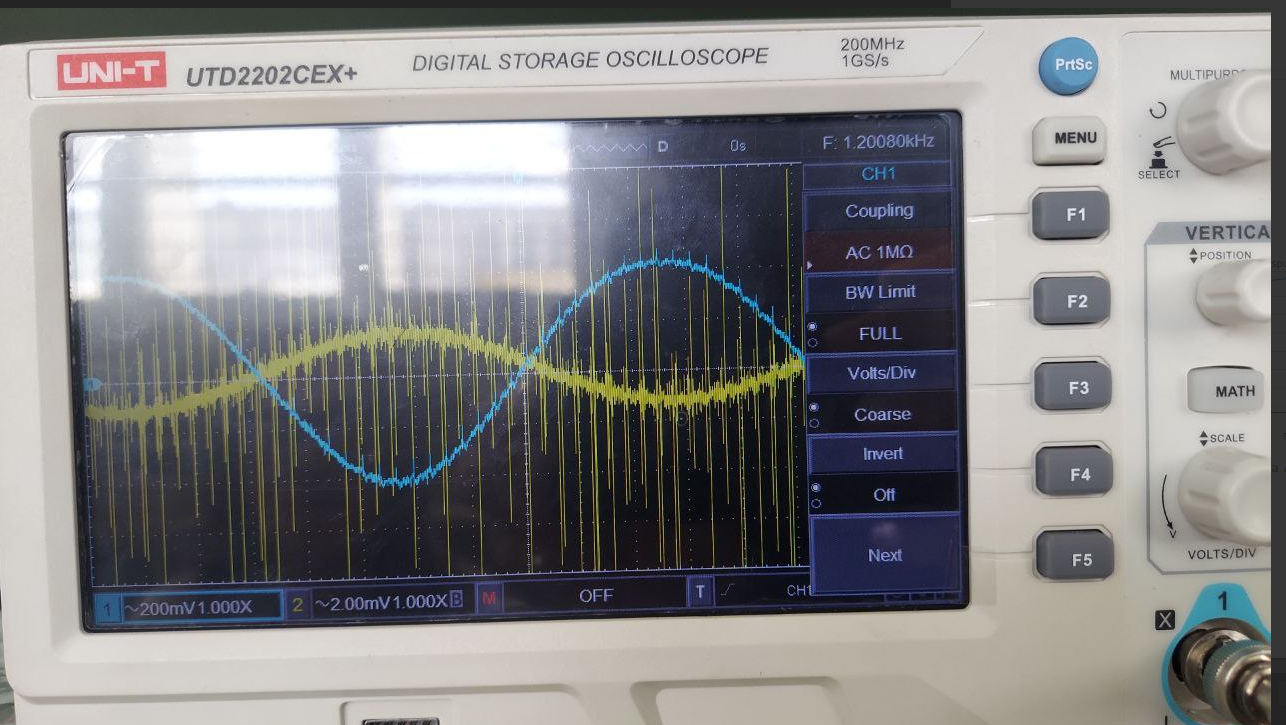
\includegraphics[width=0.8\textwidth]{src/images/resultados/p3/ganancia-etapa-impulsora.png}
    \caption{Ganancia etapa impulsora}
    \label{ilus:ganancia-etapa-impulsora}
\end{ilustracion}

\begin{ilustracion}
    \centering
    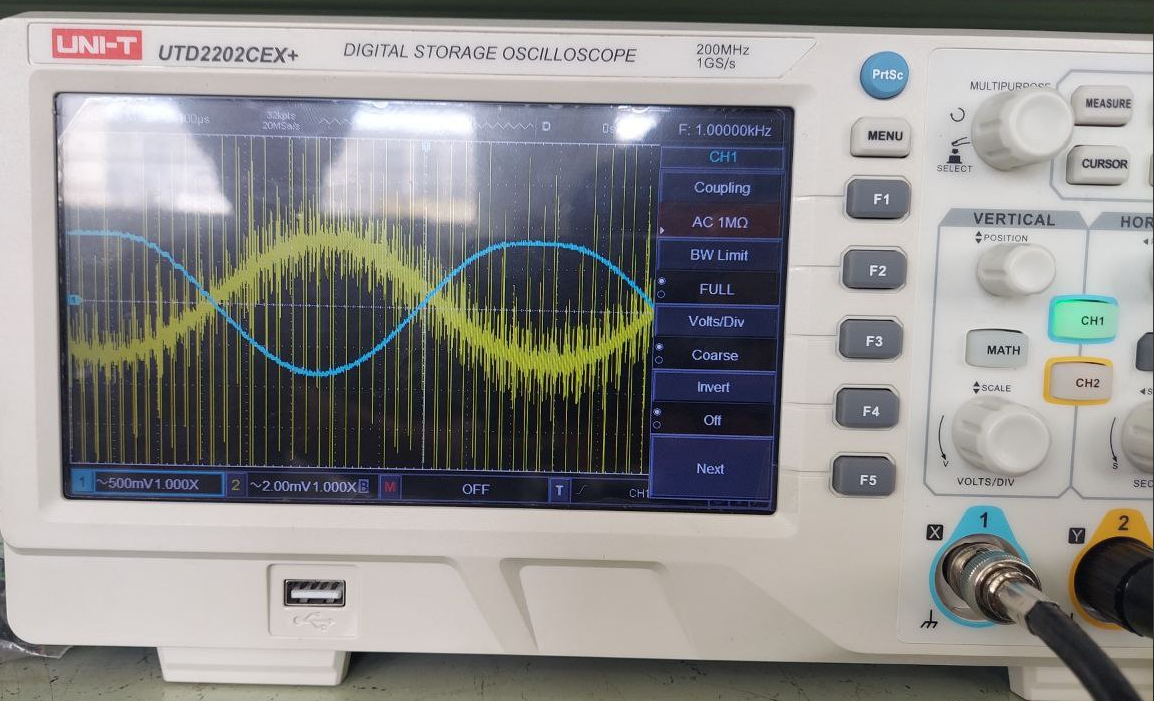
\includegraphics[width=0.8\textwidth]{src/images/resultados/p3/max-excursion-etapa-impulsora.png}
    \caption{Máxima excursión etapa impulsora}
    \label{ilus:max-excursion-etapa-impulsora}
\end{ilustracion}

\FloatBarrier
\subsubsection{Puntos de operación amplificador multietapas acoplado}

\begin{table}[h!]
\centering
\begin{tabular}{|c|c|c|c|c|c|c|c|c|c|}
\hline
\textbf{Transistor} & \textbf{\(Vc[V]\)} & \textbf{\(\varDelta Vc[V]\)} & \textbf{\(Vb[V]\)} & \textbf{\(\varDelta Vb[V]\)} & \textbf{\(Ve[V]\)} & \textbf{\(\varDelta Ve[V]\)} & \textbf{\(Re[\Omega]\)} & \textbf{\(\varDelta Re[\Omega]\)} \\ \hline
Q1 & 7.2 & 0.4 & -0.02 & 0.01 & -0.8 & 0.04 & 4700 & 235 \\ \hline
Q2 & 7.6 & 0.4 & -0.06 & 0.01 & -0.64 & 0.04 & 4700 & 235 \\ \hline
Q3 & 8 & 1 & 8 & 1 & 9 & 1 & 6800 & 340 \\ \hline
Q4 & 10 & 1 & 2 & 0.2 & 3.6 & 0.4 & 5000 & 500 \\ \hline
Q5 & 10 & 1 & 3.6 & 0.4 & 2.6 & 0.2 & 20 & 1 \\ \hline
Q6 & -10 & 1 & 2 & 0.2 & -2 & 0.2 & 20 & 1 \\ \hline
\end{tabular}
\caption{Mediciones de voltaje DC transistores en amplificador multietapas acoplado}
\label{tab:med-mediciones-voltaje-dc-transistores-amplificador-multietapas-acoplado}
\end{table}

\begin{table}[h!]
\centering
\begin{tabular}{|c|c|c|c|c|c|c|}
\hline
\textbf{Parámetro} & \textbf{Transistor} & \textbf{Valor Teórico} & \textbf{Medición} & \textbf{Incertidumbre} & \textbf{Error Absoluto} & \textbf{Error Relativo} \\ \hline
$I_{c}$ & Q1 & 0.00062 & 0.000595745 & 0.000231084 & 0.00002426 & 3.91\% \\ \hline
$I_{c}$ & Q2 & 0.00062 & 0.000510638 & 0.000230574 & 0.00010936 & 17.64\% \\ \hline
$I_{c}$ & Q3 & -0.00237 & -0.002647059 & 0.000246516 & 0.00027706 & 11.69\% \\ \hline
$I_{c}$ & Q4 & 3.02E-04 & 0.00032 & 9.49947E-05 & 0.00001764 & 5.83\% \\ \hline
$I_{c}$ & Q5 & 3.50E-04 & 0.23 & 0.018227726 & 0.22965000 & 65614.29\% \\ \hline
$I_{c}$ & Q6 & 3.50E-04 & 0.23 & 0.018227726 & 0.22965000 & 65614.29\% \\ \hline
$V_{ce}$ & Q1 & 7.79 & 8 & 0.401995025 & 0.21000000 & 2.70\% \\ \hline
$V_{ce}$ & Q2 & 7.79 & 8.24 & 0.401995025 & 0.45000000 & 5.78\% \\ \hline
$V_{ce}$ & Q3 & 2.27 & 1 & 1.414213562 & 1.27000000 & 55.95\% \\ \hline
$V_{ce}$ & Q4 & 1.24 & 6.4 & 1.077032961 & 5.16000000 & 416.13\% \\ \hline
$V_{ce}$ & Q5 & 9.99 & 7.4 & 1.019803903 & 2.59000000 & 25.93\% \\ \hline
$V_{ce}$ & Q6 & -9.99 & -8 & 1.019803903 & 1.99000000 & 19.92\% \\ \hline
\end{tabular}
\caption{Puntos estáticos de operación transistor multietapas acoplado}
\label{tab:med-puntos-estaticos-operacion-transistor-multietapas-acoplado}
\end{table}

\FloatBarrier
\subsubsection{modelo dinámico amplificador multietapas modo diferencial}

\begin{table}[h!]
\centering
\begin{tabular}{|c|c|c|c|c|c|}
\hline
\textbf{\(Vg[V]\)} & \textbf{\(\varDelta Vg[V]\)} & \textbf{\(Vi[V]\)} & \textbf{\(\varDelta Vi[V]\)} & \textbf{\(Rp[\Omega]\)} & \textbf{\(\varDelta Rp[\Omega]\)} \\ \hline
0.52 & 0.01 & 0.17 & 0.01 & 42000 & 4200 \\ \hline
\end{tabular}
\caption{Mediciones impedancias de entrada circuito multietapas modo diferencial}
\label{tab:med-impedancias-entrada-circuito-multietapas-modo-diferencial}
\end{table}

\begin{table}[h!]
\centering
\begin{tabular}{|c|c|c|c|c|c|}
\hline
\textbf{\(Vo_{sc}[V]\)} & \textbf{\(\varDelta Vo_{sc}[V]\)} & \textbf{\(Vo_{cc}[V]\)} & \textbf{\(\varDelta Vo_{cc}[V]\)} & \textbf{\(Rp[\Omega]\)} & \textbf{\(\varDelta Rp[\Omega]\)} \\ \hline
0.52 & 0.04 & 0.32 & 0.02 & 100 & 5 \\ \hline
\end{tabular}
\caption{Mediciones impedancia de salida amplifiador multietapa}
\label{tab:med-impedancia-salida-amplifiador-multietapa}
\end{table}

\begin{table}[h!]
\centering
\begin{tabular}{|c|c|c|c|}
\hline
\textbf{\(Vi[V]\)} & \textbf{\(\varDelta Vi[V]\)} & \textbf{\(Vo[V]\)} & \textbf{\(\varDelta Vo[V]\)} \\ \hline
0.0036 & 0.0002 & 0.52 & 0.04 \\ \hline
\end{tabular}
\caption{Ganancia amplificador multietapas modo diferencial}
\label{tab:med-ganancia-amplificador-multietapas-modo-diferencial}
\end{table}


\begin{table}[h!]
\centering
\begin{tabular}{|c|c|c|c|c|c|}
\hline
\textbf{Parámetro} & \textbf{Valor} & \textbf{Medición} & \textbf{Incertidumbre} & \textbf{Error Absoluto} & \textbf{Error Relativo} \\ \hline
$[Z] d$ & 43,990 & 20400 & 2771.263618 & 23590 & 53.63\% \\ \hline
$[Z] o$ & 132 & 62.5 & 16.40625 & 69.5 & 52.65\% \\ \hline
$[A]$ & 379.22 & 144.444444444444 & 13.70592797 & 234.7755556 & 61.91\% \\ \hline
\end{tabular}
\caption{Modelo dinámico amplificador multietapas modo diferencial}
\label{tab:med-modelo-dinamico-amplificador-multietapas-modo-diferencial}
\end{table}

\begin{ilustracion}[ht]
    \centering
    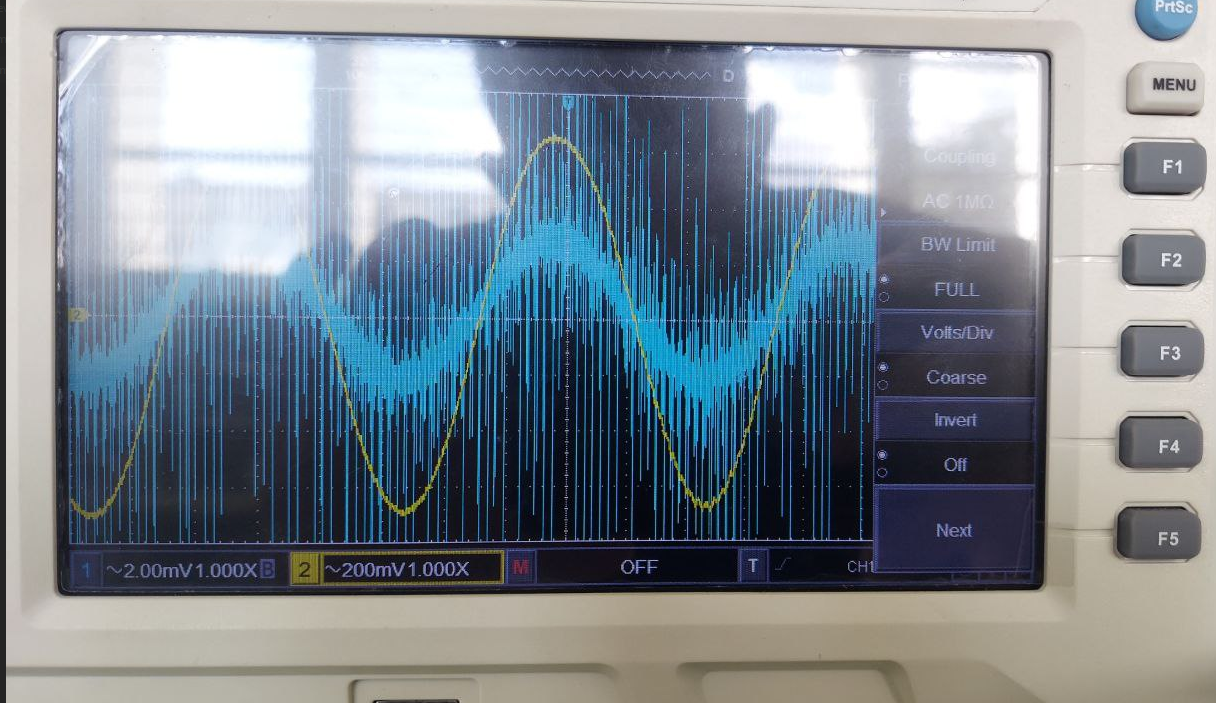
\includegraphics[width=0.8\textwidth]{src/images/resultados/p3/ganancia-multietapas-mod-diff.png}
    \caption{Ganancia del modelo dinámico amplificador multietapas modo diferencial}
    \label{ilus:ganancia-multietapas-mod-diff}
\end{ilustracion}

\begin{ilustracion}[ht]
    \centering
    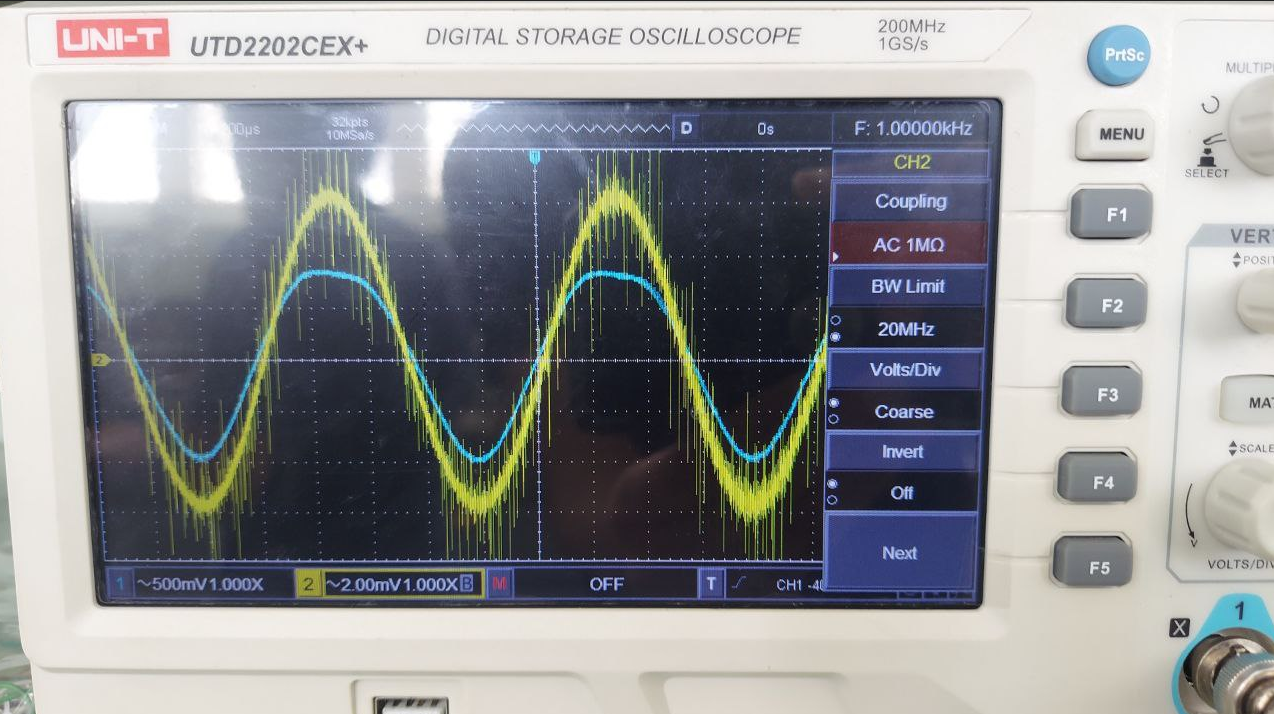
\includegraphics[width=0.8\textwidth]{src/images/resultados/p3/max-excursion-multietapas-mod-diff.png}
    \caption{Máxima excursión del modelo dinámico amplificador multietapas modo diferencial}
    \label{ilus:med-max-excursion-multietapas-mod-diff}
\end{ilustracion}

\FloatBarrier
\subsubsection{modelo dinámico amplificador multietapas modo común}

\begin{table}[h!]
\centering
\begin{tabular}{|c|c|c|c|c|c|}
\hline
\textbf{\(Vg[V]\)} & \textbf{\(\varDelta Vg[V]\)} & \textbf{\(Vi[V]\)} & \textbf{\(\varDelta Vi[V]\)} & \textbf{\(Rp[\Omega]\)} & \textbf{\(\varDelta Rp[\Omega]\)} \\ \hline
0.032 & 0.004 & 0.008 & 0.0004 & 20000 & 1000 \\ \hline
\end{tabular}
\caption{Impedancia de entrada amplificador multietapas modo común}
\label{tab:med-impedancia-entrada-amplificador-multietapas-modo-comun}
\end{table}


\begin{table}[h!]
\centering
\begin{tabular}{|c|c|c|c|}
\hline
\textbf{\(Vi[V]\)} & \textbf{\(\varDelta Vi[V]\)} & \textbf{\(Vo[V]\)} & \textbf{\(\varDelta Vo[V]\)} \\ \hline
0.024 & 0.002 & 0.38 & 0.02 \\ \hline
\end{tabular}
\caption{Ganancia amplificador multietapas modo común}
\label{tab:med-ganancia-amplificador-multietapas-modo-comun}
\end{table}

\begin{table}[h!]
\centering
\begin{tabular}{|c|c|c|c|c|c|}
\hline
\textbf{Parámetro} & \textbf{Valor} & \textbf{Medición} & \textbf{Incertidumbre} & \textbf{Error Absoluto} & \textbf{Error Relativo} \\ \hline
$[Z] d$ & 49000 & 41142.85714 & 5974.907966 & 7857.142857 & 16.03\% \\ \hline
$[Z] o$ & 132 & 62.5 & 602.0083575 & 69.5 & 52.65\% \\ \hline
$[A]$ & 40.05 & 15.83333333 & 1.560569795 & 24.21666667 & 60.47\% \\ \hline
\end{tabular}
\caption{Modelo dinámico amplificador multietapas modo común}
\label{tab:med-modelo-dinamico-amplificador-multietapas-modo-comun}
\end{table}

\begin{ilustracion}
    \centering
    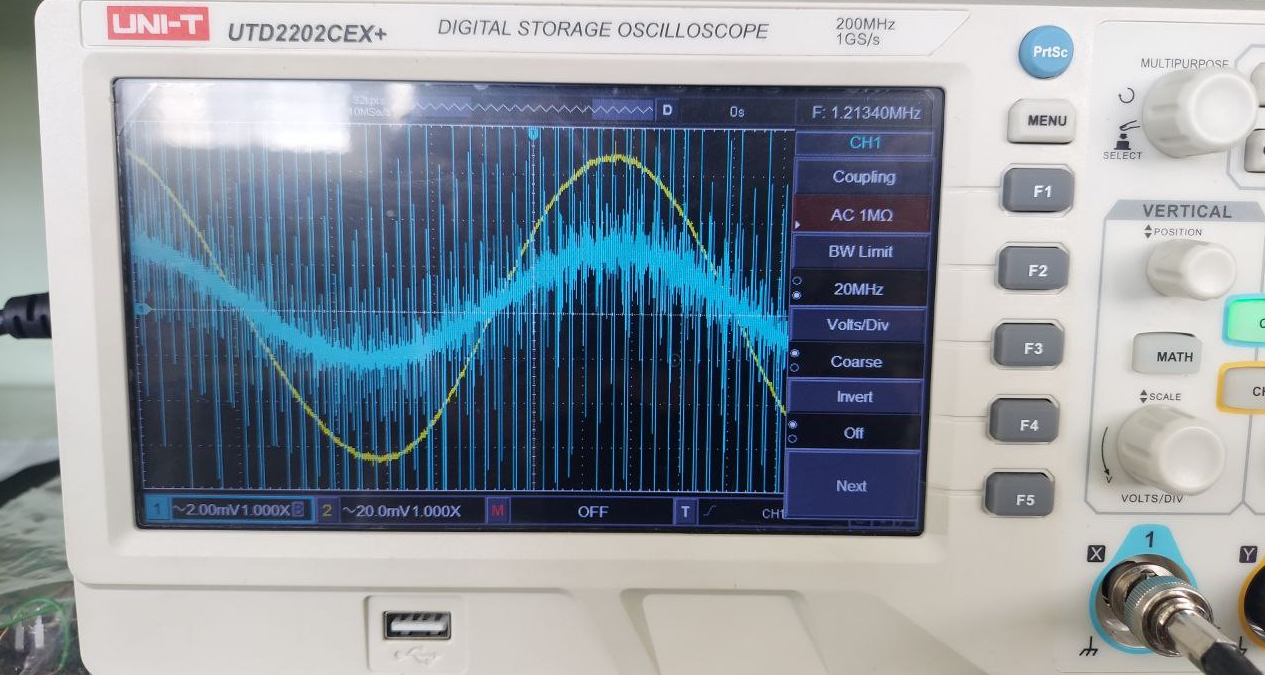
\includegraphics[width=0.8\textwidth]{src/images/resultados/p3/ganancia-multietapas-mod-comun.png}
    \caption{Ganancia del modelo dinámico amplificador multietapas modo común}
    \label{ilus:ganancia-multietapas-mod-comun}
\end{ilustracion}

\begin{ilustracion}[ht]
    \centering
    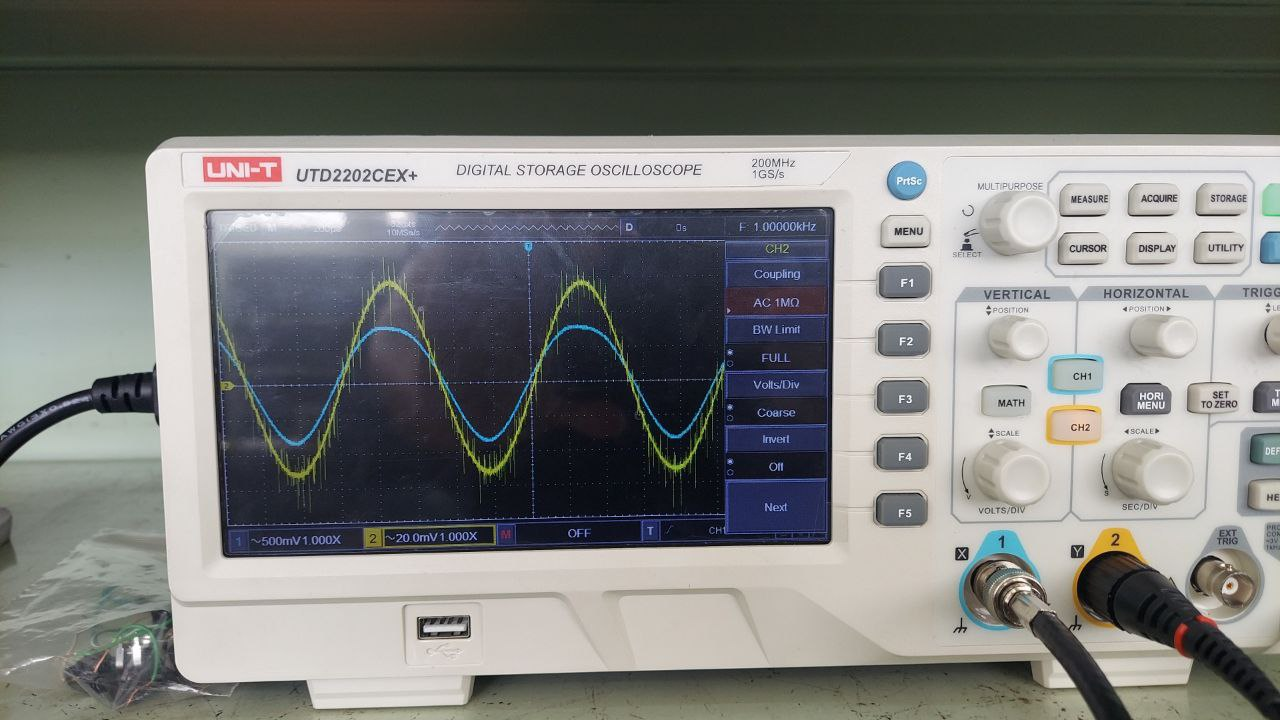
\includegraphics[width=0.8\textwidth]{src/images/resultados/p3/max-excursion-multietapas-mod-comun.png}
    \caption{Máxima excursión del modelo dinámico amplificador multietapas modo común}
    \label{ilus:med-max-excursion-multietapas-mod-comun}
\end{ilustracion}

